%
% File: Direxeno.tex
% Author: Ran Itay
% Description: Direxeno experiment
%
\let\textcircled=\pgftextcircled
\chapter{Direxeno}
\label{chap:Direxeno}
\initial{I}n Liquid Xenon experiments, the cloud of excimers produced when a particle recoils energy in xenon is estimated to have a complex shape. Nonetheless it is expected to have a typical size of O(100nm). Hence it is expected that the excimer cloud might undergo a \superradiance emission. A variation in the temporal time of radiation between ERs and NRs might exist due to the size of the excimer cloud. This can improve the discrimination between background(ER) and signal(NR) for LXe DM detectors. Moreover weather the emitted radiation is correlated to the incoming exciting particle momentum, can be a more powerful tool for background reduction. Discarding events coming from the direction of the sun for example, is necessary once the neutrino floor(TODO add cite neutrino floor) will be crossed.  

Early studies conducted by Basov~\citep{BasovSRTheory} (experimentally) and in NIST~\cite{stim} (theoretically) both present the option of generating a coherent radiation in the VUV regime (~178nm). The experimental setup was designed to bombard the LXe with 800~\,keV electron current pulse exciting (10\,ns) the LXe. The constant electron current causes a reverse population constantly. In contrary in direct detection of DM experiments, there is no "pump" producing this inverse population. The study of weather a cloud of excimers caused by a single interaction can exhibit \superradiance is still absence.

In this chapter we discuss Direxeno (Directional Xenon). An experimental setup designed at measuring \superradiance or any other non-linear effect in LXe.

\section{Experimental Setup}
\label{expSetup}

%%%%%%%%%%%%%%%%%%%%%%%%%%%%%%%%%%%%%%%%%%%%%%%%%%%%%%%%%%%%%%%%%%%%%%%%%%%%%%%%%%%%%%%%%%%%%%%%%%%%%%%%%%%%%%%
%Initiator: Ran Itay
%Last modified by: MM Devi, May 26 2017
%Comment: The detector section has been modified. MMdevi's changes are made in blue
%%%%%%%%%%%%%%%%%%%%%%%%%%%%%%%%%%%%%%%%%%%%%%%%%%%%%%%%%%%%%%%%%%%%%%%%%%%%%%%%%%%%%%%%%%%%%%%%%%%%%%%%%%%%%%%

In order to identify superradiance effects in LXe, the temporal and spatial properties of scintillation events should be studied and quantified. In the DireXeno system LXe is circulated through a small spherical cavity held in a thick sphere made of high purified fused silica (HPFS). The sphere is surrounded ($\sim4\pi$) by PMTs allowing high resolution spatial and temporal measurements of individual photons. The PMTs do not come in contact with the xenon, so less impurities are introduced to it, and the material selection is less stringent. The geometrical design of the system approximates a point  source of scintillation photons, and a detailed vertex reconstruction within the LXe bubble is unnecessary. A schematic view of the system is shown in Fig~\ref{fig:detSch} . 

\begin{figure}[h]
\centerline{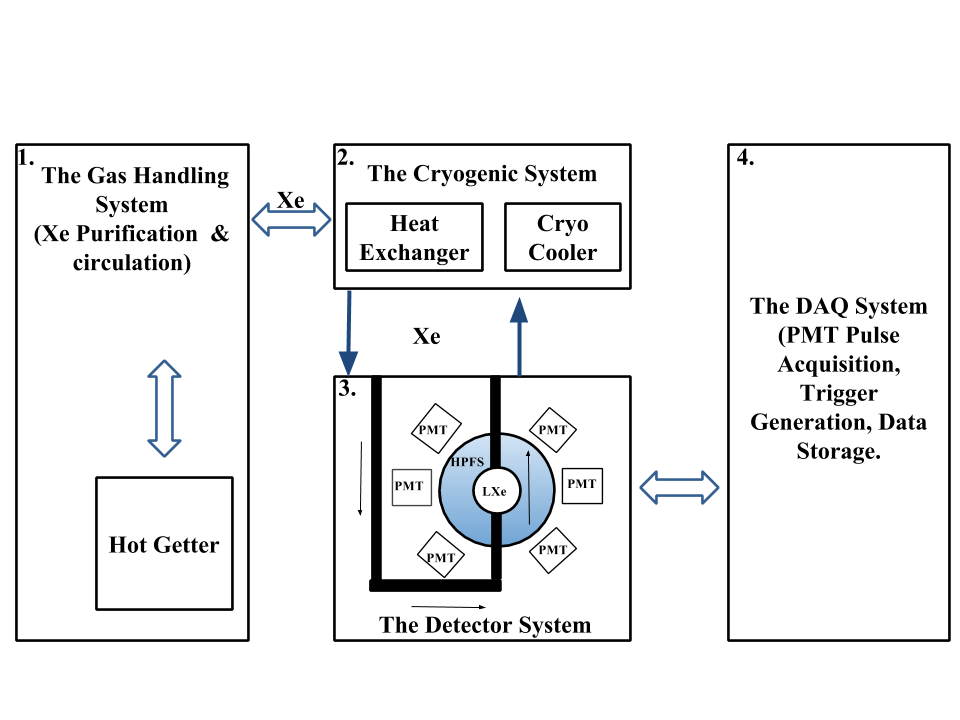
\includegraphics[width=0.8\linewidth]{fig/DetSch.png}}
\caption{A schematic view of DireXeno.}
\label{fig:detSch}
\end{figure}


The current system is designed with \RanComment{TODO check digitzation time} $\sim1$\,ns time resolution, less than $1$\,ns synchronization between PMTs, and $\sim8$ radians spatial resolution. Since the exact nature and magnitude of superradiance in LXe is yet unknown a guiding principle in the design was flexibility to upgrades or redesign of any part of the system to fulfill any future experiment requirements. The modular design allows gain fast and easy recovery in case of components malfunction.

The system is made of four main building blocks. (i) \textbf{The gas handling system} which in normal working mode circulates the xenon and purifies it. (ii) \textbf{The cryogenic system}, liquefies the xenon and 
delivers it to the detector system. (iii) \textbf{The detector system} consists of a fused silica sphere that 
holds a small bubble of LXe target, and PMTs around the sphere. (iv) \textbf{The DAQ system} supplies high voltage (HV) 
to the PMTs and handles monitoring, triggering and digitization of data. The entire assembly is held on 3 separate racks as shown in Fig.~\ref{fig:fulldet}.



\begin{figure}[h]
\centerline{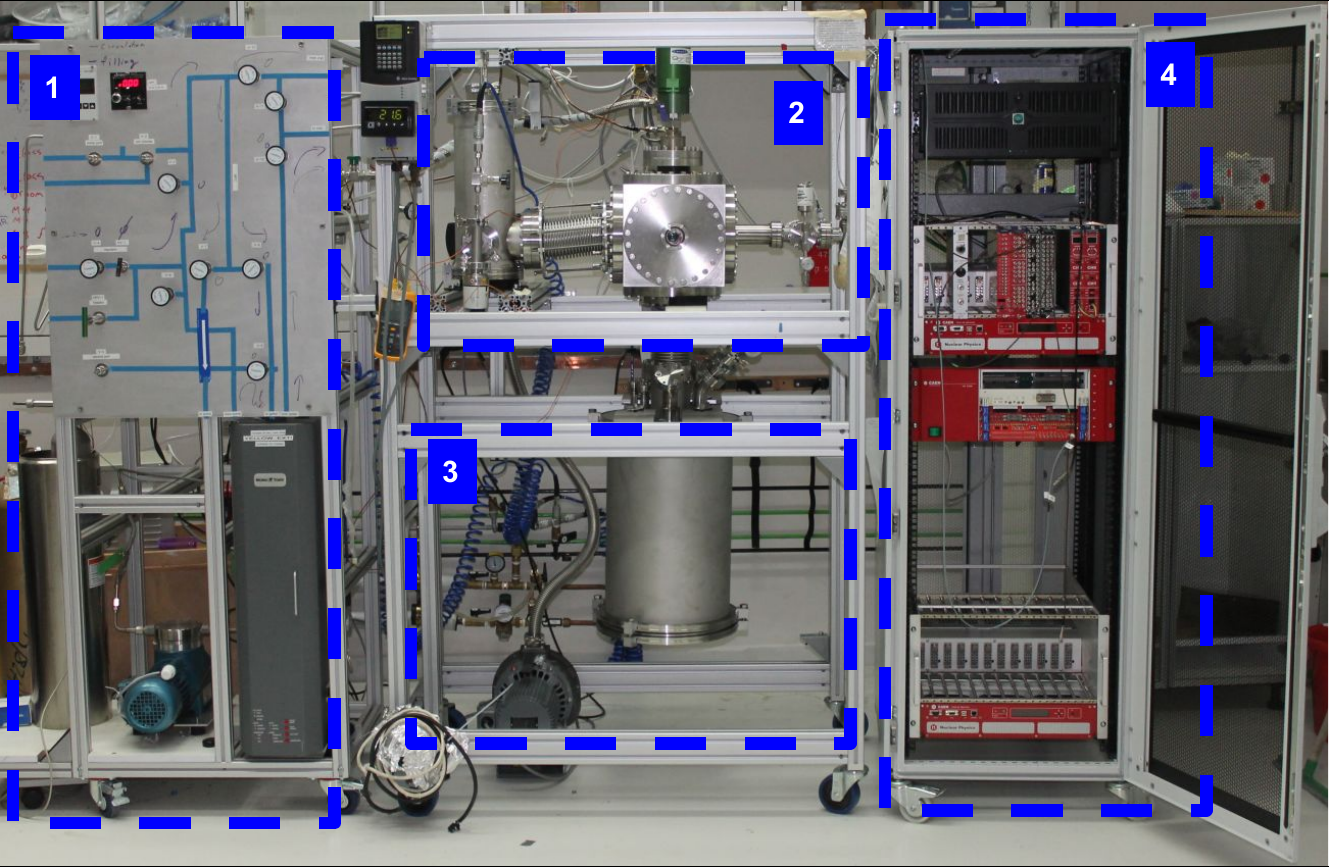
\includegraphics[width=0.8\linewidth]{fig/FullSys.png}}
\mycaption[The DireXeno system]{The DireXeno system mounted on the three racks. 1. The gas handling system. 2. The cryogenic system including the heat exchanger. 3. The detector chamber. 4. The Data acquisition system.
\label{fig:fulldet}}
\end{figure}



\subsection{The gas handling system}
\label{subsec:gas}

In DIREXENO only the prompt scintillation is measured, so a high level of LXe purity is not of a great importance. However in many LXE detectors the desired level of impurity concentration is at the level of 1 ppb $O_2$ equivalent~\cite{Aprile:2009dv} This is crucial to allow 
ionization electrons drift for several cm. To reach that purity level in a reasonable amount 
of time (several days instead of months), 
a continuous purification is needed. The gas handling system provides this process along 
with all gas handling operations such as filling and recuperation and circulation. The xenon circulation also plays a major role in heat transfer.


During purification, The xenon is forced by a circulation pump\footnote{N143 SN.12E AC 230V50HZ KNF diaphragm circulation pump} extracting LXe from the detector part through a heat exchanger\footnote{GEA GBS100M-24 plate heat exchanger} 
where it is heated and vaporized, into a hot getter\footnote{MONO-TORR PS4-MT15-R-2} which cleans the xenon. The xenon passes through a mass flow controller\footnote{MKS mass flow controller 1179A00614CR1BM} (MFC), 
enabling monitoring and controlling the amount of heat introduced to the system.  Once purified, the xenon is delivered back to the cryogenic system 
via the heat exchanger, where the remaining GXe is 
liquefied before flowing back to the detector part. A schematic of this 
system is shown in fig.~\ref{fig:gasSchematic}.


%%%%%%%%%%%%%%%%%%%%%%%%%%%%%%%%%%%%%%%%%%%%%%%%%%%%%%%%%%%%%%%%%%%%%%%%%%%%%%%%%%
\begin{figure}[h]
\centerline{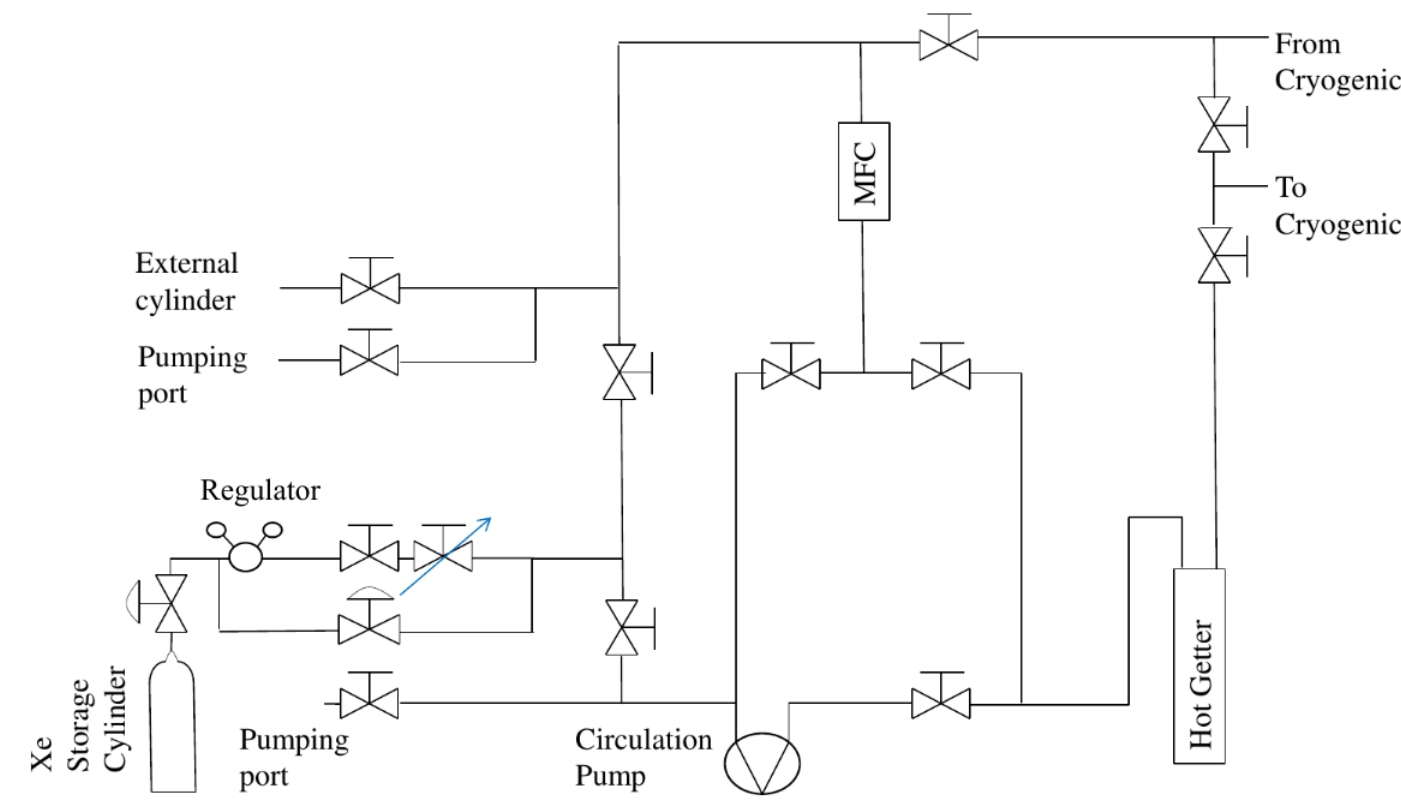
\includegraphics[width=0.75\linewidth]{fig/GasSchematics.png}}
\mycaption[DireXeno gas schematics]{Schematics of the gas handling system. High pressure valves are indicated as 
valves with arcs. Needle valves are indicated as 
a valve with an arrow.
\label{fig:gasSchematic}}
\end{figure}
%%%%%%%%%%%%%%%%%%%%%%%%%%%%%%%%%%%%%%%%%%%%%%%%%%%%%%%%%%%%%%%%%%%%%%%%%%%%%%%%%%


\subsection{The cryogenic system}
\label{subsec:cryo}

Remote cooling is generally used in LXe experiments due to reduction in background radiation and acoustic noise from the cooler to the detector, and due to design flexibility. The cryogenic system is connected to the gas handling system on 
one side and to the detector part on the other, and built such that replacing the cryo-cooler type (e.g., to PTR) requires just an adaptation to the top flange.


The cryogenic system is divided to an outer vessel (OV) which holds 
the insulation vacuum, and an inner vessel (IV) which holds the xenon. In addition to the vacuum which prevents heat leakage due to diffusion and convection, the IV is completely covered by multi layer aluminized Myler to prevent heating via radiation.  

%%%%%%%%%%%%%%%%%%%%%%%%%%%%%%%%%%%%%%%%%%%%%%%%%%%%%%%%%%%%%%%
\begin{figure}
\centering
\begin{minipage}[c]{0.35\textheight}
\subbottom[]{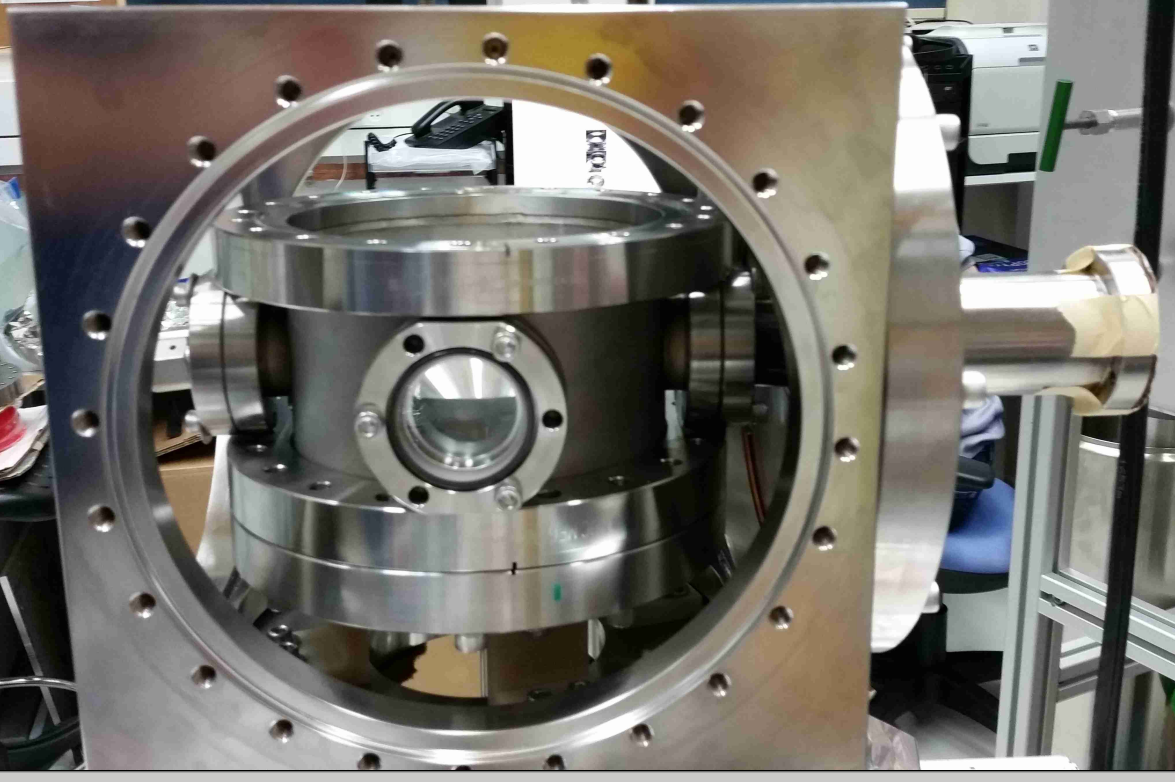
\includegraphics[width=\textwidth]{fig/cryoOpenCrop.png}}
\end{minipage}
\begin{minipage}[c]{0.45\textheight}
\subbottom[]{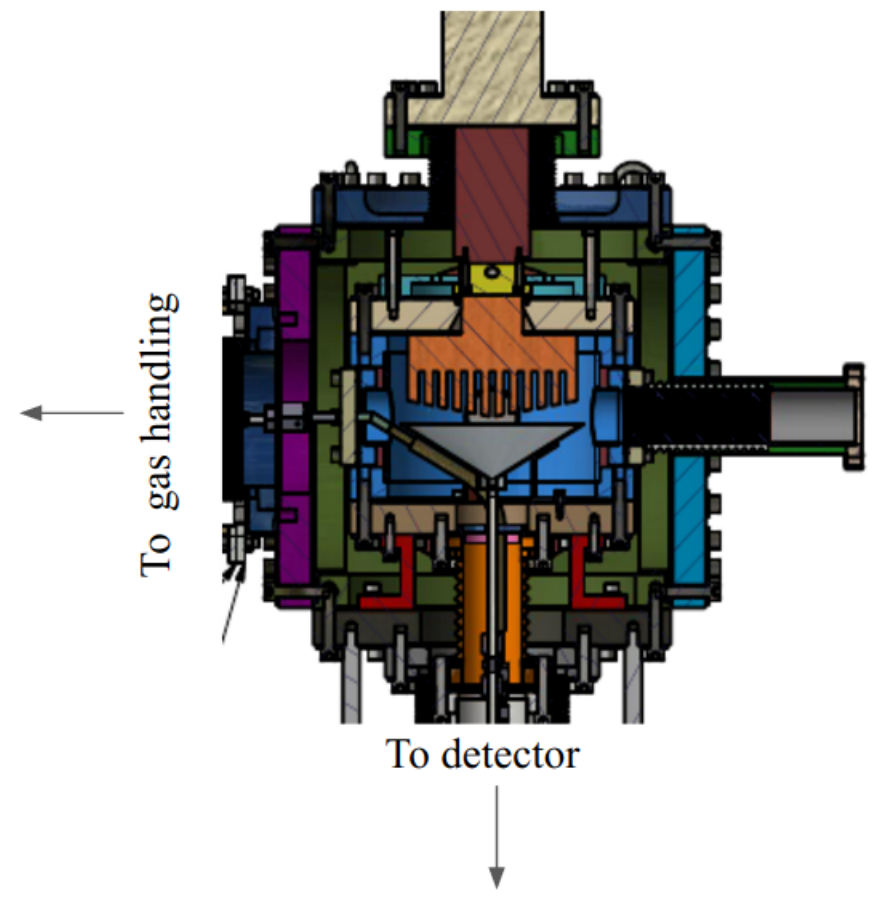
\includegraphics[width=\textwidth]{fig/cryoMirror.png}}
\end{minipage}
\mycaption[The cryogenic system]{(a) Picture of the cryogenic system. (b) CAD view of the cryogenic system.  
\label{fig:cryo}}
\end{figure}
%%%%%%%%%%%%%%%%%%%%%%%%%%%%%%%%%%%%%%%%%%%%%%%%%%%%%%%%%%%%%%%%

The OV is made of a 10" Conflat (CF) cube, with ports on all six faces, interfacing the gas handling system and  the detector part, and bearing service ports (e.g., feed-throughs, pumping ports, 
view ports). The OV is connected to the detector part via a 6" CF flexible bellows, providing a shared vacuum.

The IV is made of 1.5" long cylinder with 6" CF flanges on both sides, holding xenon within. A 120~\,mm diameter cold finger is welded to its top flange. The design of the cold finger is similar to the one in~\cite{xe100_instr2012}. The inner part of the cold finger is made of long fins, resulting in a better heat transport.  The upper part of the cold finger is in thermal contact with the 
QDrive cryo-cooler~\footnote{QDrive 20BB 9p6 A 3 AYNBNCO} via a copper adapter. The copper adapter 
holds two $100\Omega$ pt resistor which are connected to a PID reader\footnote{cryo-con model 
18i Cryogenic Temp Monitor} for temperature measurements. A cartridge-heater 
is also inserted to the copper adapter for emergency heating in case xenon freezes on the 
cold finger. 

The cryo-cooler is connected via a $4\frac{1}{2}$" 
flange to the OV top flange. While usually cryo-coolers used for 
xenon experiments constantly operate in maximal cooling, the QDrive cryo-cooler utilizes a 
temperature control to vary its cooling power up to 70\,W. This allows setting a desired working temperature which is constant within less then $0.1~\mathrm{^{\circ}C}$ measured on the cryo-cooler.

On the inner side of the IV bottom flange a thin 0.6~mm SS funnel is installed 
collecting LXe drops from the cold finger, and delivering them to the  detector. This flange is attached to the detector part, via a $3\frac{3}{8}$" flexible bellows. The 
bellows hosts two pipes connected to the circulation system, and a third pipe coming 
from the funnel. The three pipes deliver LXe whereas the GXe is filling the bellows volume. The purer LXe (from the gas handling system) and the less pure LXe (from the cold finger) are separated, and can be delivered to different parts of the system. Some of the guidelines for the design of 
the cryogenic system are based on~\cite{Giboni}. The CAD view of 
the design of the cryogenic system and a photo of the actual system are shown in Fig~\ref{fig:cryo}. 

%%%%%%%%%%%%%%%%%%%%%%%%%%%%%%%%%%%%%%%%%%%%%%%%%%%%%%%%%%%%%%%%%%%%%%%%%%%%%%%%%%%%%%%%%%%%%%%%%%%%%%%%%%%%%%%%%%%%%%%%%%%%%%%%%%%%%%%%%%%%%%%%%%%%%%%%%%%%%
\subsection{The detector system}
\label{subsec:det}
 
The detector system refers to a vacuum chamber and its inner assembly consisting of a transparent sphere that 
contains the LXe, the PMT sensors observing it and their accessories. This chamber is placed below the cryogenic system. 


The interface unit to the cryogenic system is built out of two flanges welded together via seven tubes, which serve as service ports for electrical and other feedthroughs: four 
with a $2 \frac{3}{4}/$ CF flange, and three with a $1\frac{1}{3}$ CF flange (mini-CF). 
The upper flange, ISO-K NW320, shares the cryogenic system's OV insulation vacuum, while the bottom one, CF-10", is part of the IV and could hold xenon for future detectors. 
The CF flange is also adapted to fit a smaller CF-$4\frac{5}{8}$" flange which is currently used.

The vacuum chamber is made of an ISO-K NW320 nipple closed with a blank flange from below, 
the length of the nipple is determined such that the maximal height of the whole 
apparatus is 190~\,cm, allowing an easy transport of the detector through standard doors.
 
The $4\frac{5}{8}$" CF flange is connected to a split vessel that serves as a LXe reservoir. one part is connected 
to the top of the HPFS sphere, and one to the bottom. LXe is circulated such that LXe coming from the gas system drips into one part and pumped from the other. This controls the liquid level, and the sphere is constantly filled with LXe. 


The sphere is a custom designed hollow shell made of Corning HPFS 8655 with high transmittance to VUV. Two Invar tubes with SS mini-CF flange are connected to the sphere on both sides. The technical design and photo of the sphere are shown in Fig.~\ref{fig:sphere}. The optical properties of the sphere will be further discussed in Sec.~\ref{sec:opt}. 
The bottom flange of the sphere is held using a brass holder to prevent 
force or torque applied on the sphere while mounting it. The 
brass holder is connected to a plate held from the top CF-10" flange. 



%%%%%%%%%%%%%%%%%%%%%%%%%%%%%%%%%%%%%%%%%%%%%%%%%%%%%%%%%%%%%%%%%%%%%%
\begin{figure}
\centering
\begin{minipage}[c]{0.6\textheight}
\centering
\subbottom[]{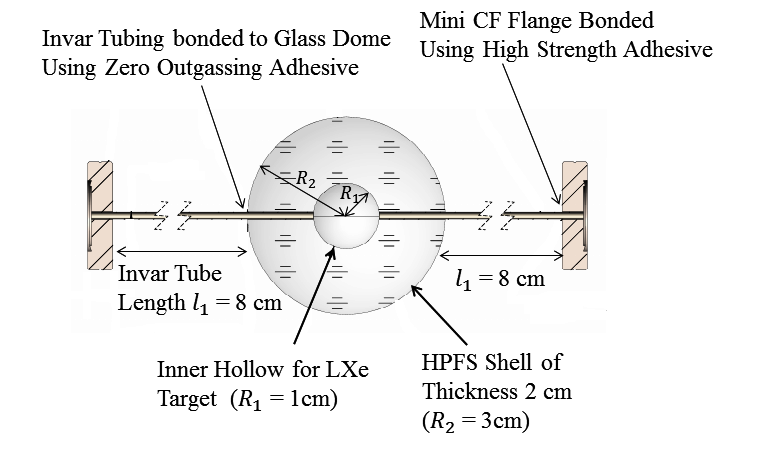
\includegraphics[width=\textwidth]{fig/spheredesign1.png}}
\end{minipage}
\begin{minipage}[c]{0.35\textheight}
\centering
\subbottom[]{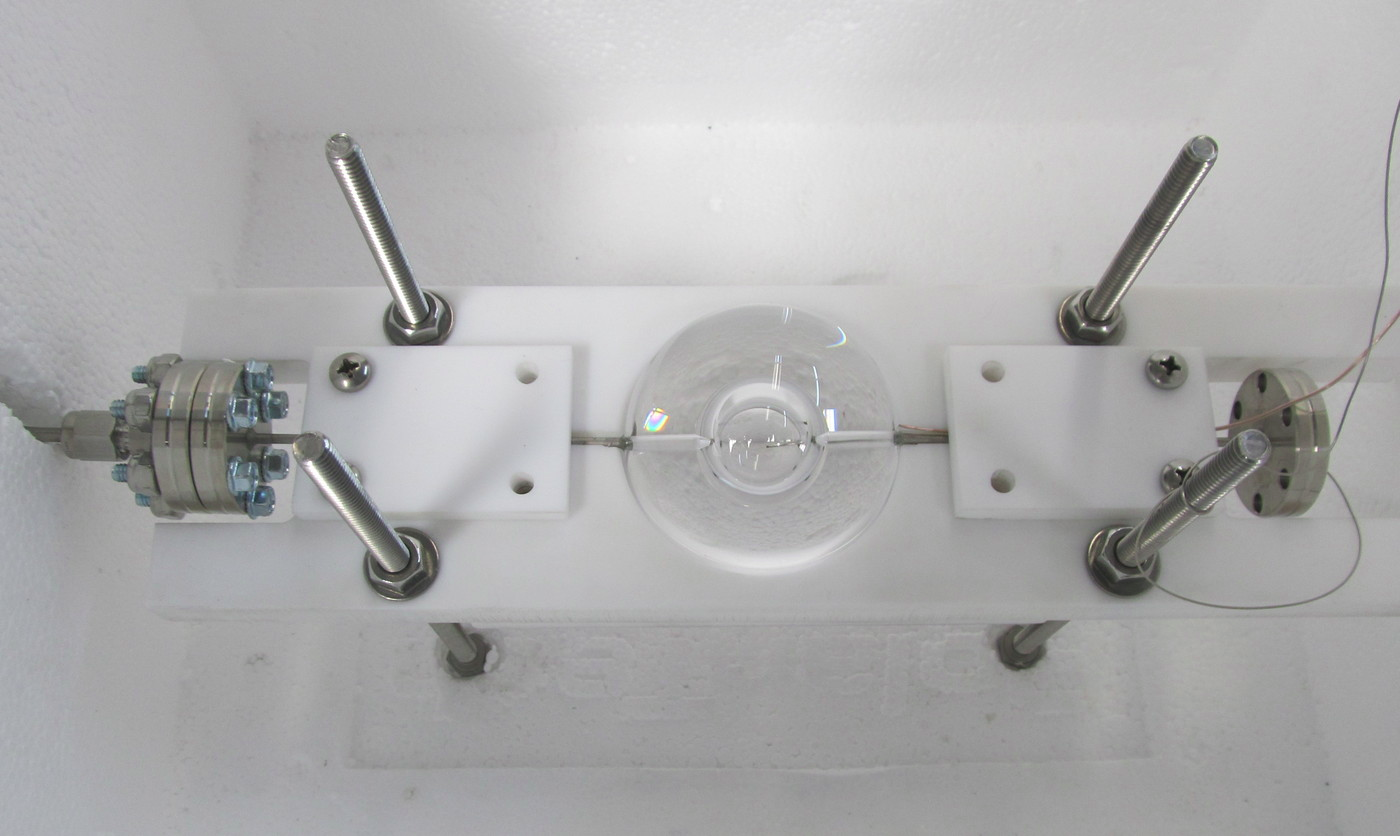
\includegraphics[width=\textwidth]{fig/spherephoto.png}}
\end{minipage}
\mycaption[The HPFS shell]{(a) The technical design of the HPFS shell with Invar tubing and mini CF flanges. 
(b) The manufactured HPFS shell, held in a test fixture. 
\label{fig:sphere}}
\end{figure}
%%%%%%%%%%%%%%%%%%%%%%%%%%%%%%%%%%%%%%%%%%%%%%%%%%%%%%%%%%%%%%%%%%%%%%%



Photons emitted from the LXe in the sphere are detected by 20  PMTs\footnote{R8520-406 Hamamatsu 1" PMT, active area 20.5 mm $\times 20.5 mm$}. 
The PMTs are chosen to have a quantum efficiency greater than 30\% at 178\,nm. The gain of the PMTs is ~ 2 $\times$ 10$^6$ at an applied voltage of 900\,V . A positive voltage divider\footnote{Hamamatsu VDS18130p 24 channel poisitve polarity.}, is used to to provide high voltage to the PMTs. 
The PMTs are held with a special aluminum holder, coated with anti-reflection substance. 
The holder is made of two hemispheres hosting the PMTs in 3 rows all of them pointing to the 
center of the sphere. The PMTs are attached to the holder by their voltage--divider bases using M2 PEEK screws (see Fig~\ref{fig:pmtholder}). 
The CAD design and a photo of the detector system are shown 
in Fig.~\ref{fig:detector}.

%%%%%%%%%%%%%%%%%%%%%%%%%%%%%%%%%%%%%%%%%%%%%%%%%%%%%%%%%%%%%%%%%%%%%%%%%%%%%%%%%%%%%%%%%%%
\begin{figure}[]
   \centering
   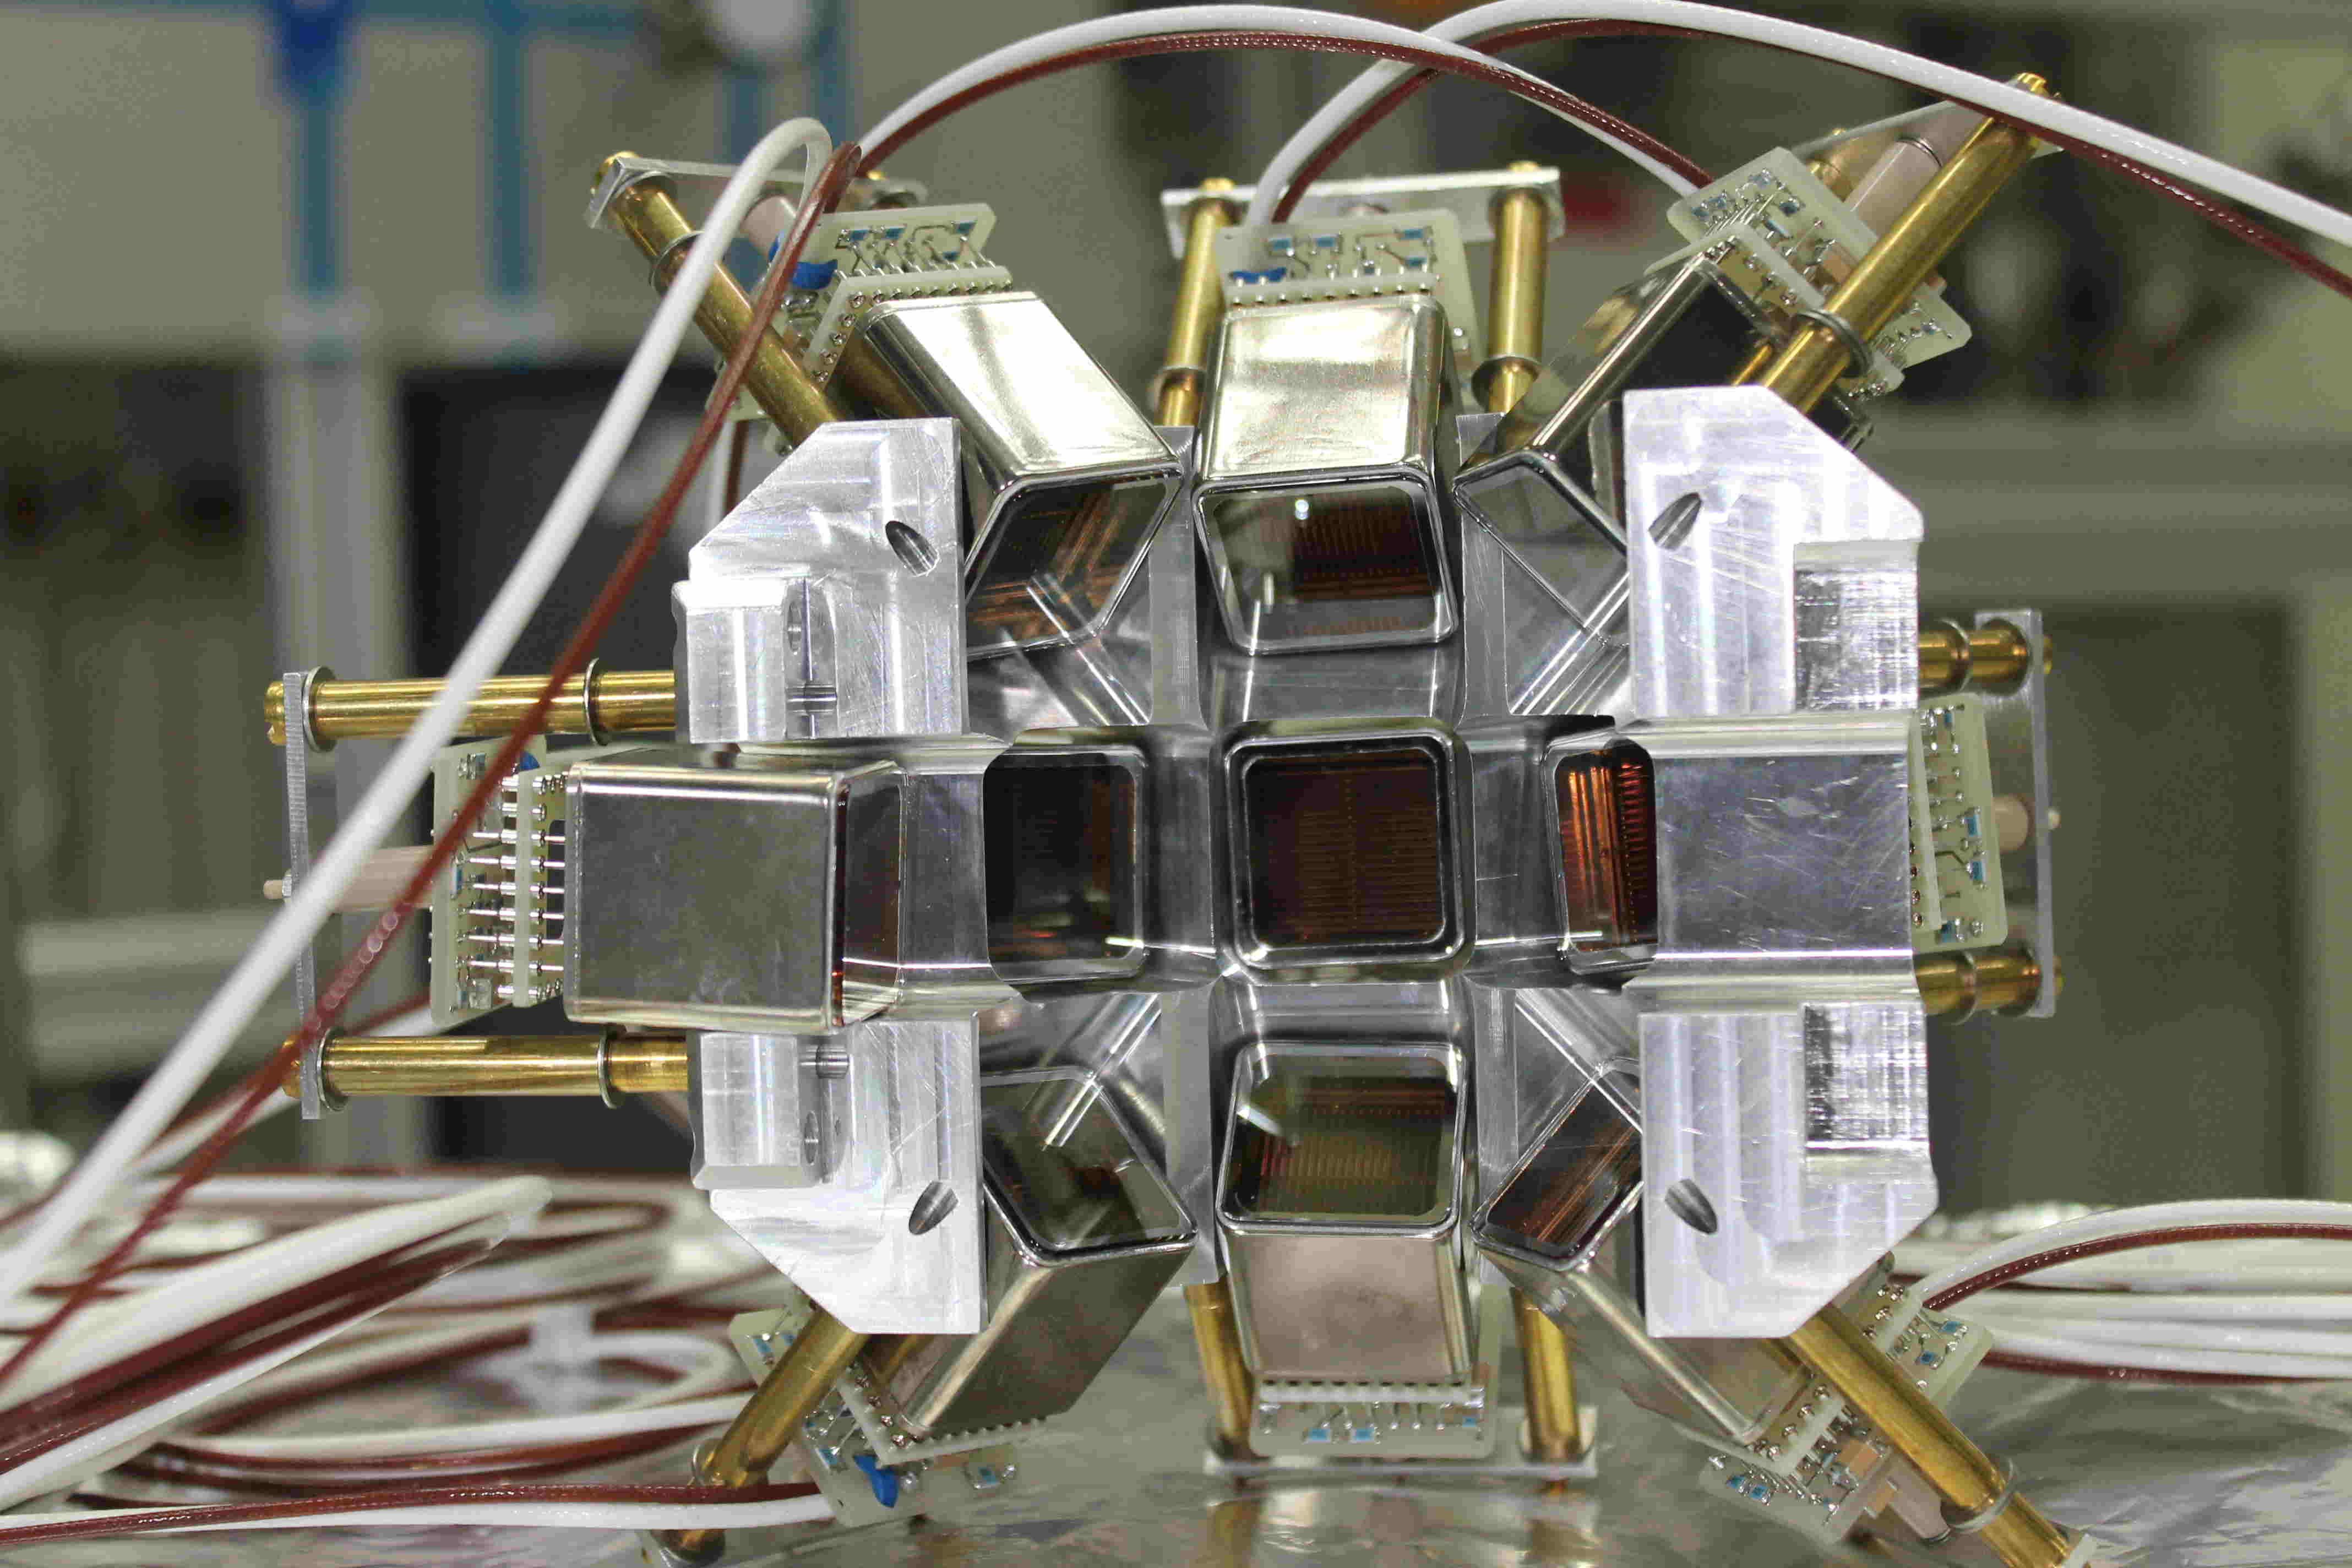
\includegraphics[width=0.7\textwidth]{fig/PMTholder.JPG}
   \mycaption[PMT holder]{A PMT holder--hemisphere. Two identical hemispheres are used to hold the PMTS around the sphere.} 
   \label{fig:pmtholder}
\end{figure}
%%%%%%%%%%%%%%%%%%%%%%%%%%%%%%%%%%%%%%%%%%%%%%%%%%%%%%%%%%%%%%%%%%%%%%%%%%%%%%%%%%%%%%%%%%%

%%%%%%%%%%%%%%%%%%%%%%%%%%%%%%%%%%%%%%%%%%%%%%%%%%%%%%%%%%%%%%%%%%%%%%%%%%
\begin{figure}[h]
\centering
\begin{minipage}[c]{0.55\textwidth}
\subbottom[]{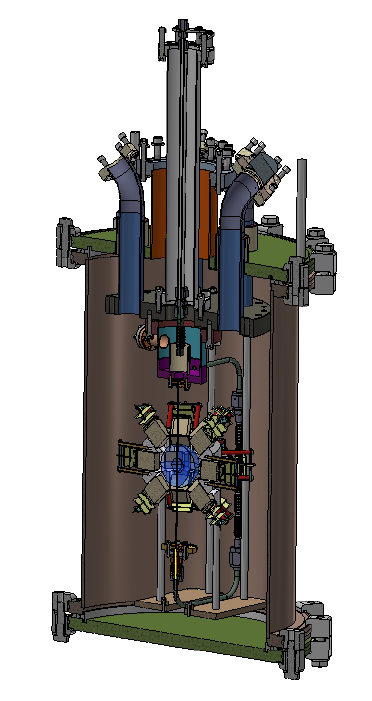
\includegraphics[width=0.75\textwidth , height=0.4\textheight]{fig/detCAD.png}}% Here is how to import 
\end{minipage}	
\begin{minipage}[c]{0.45\textwidth}
\subbottom[]{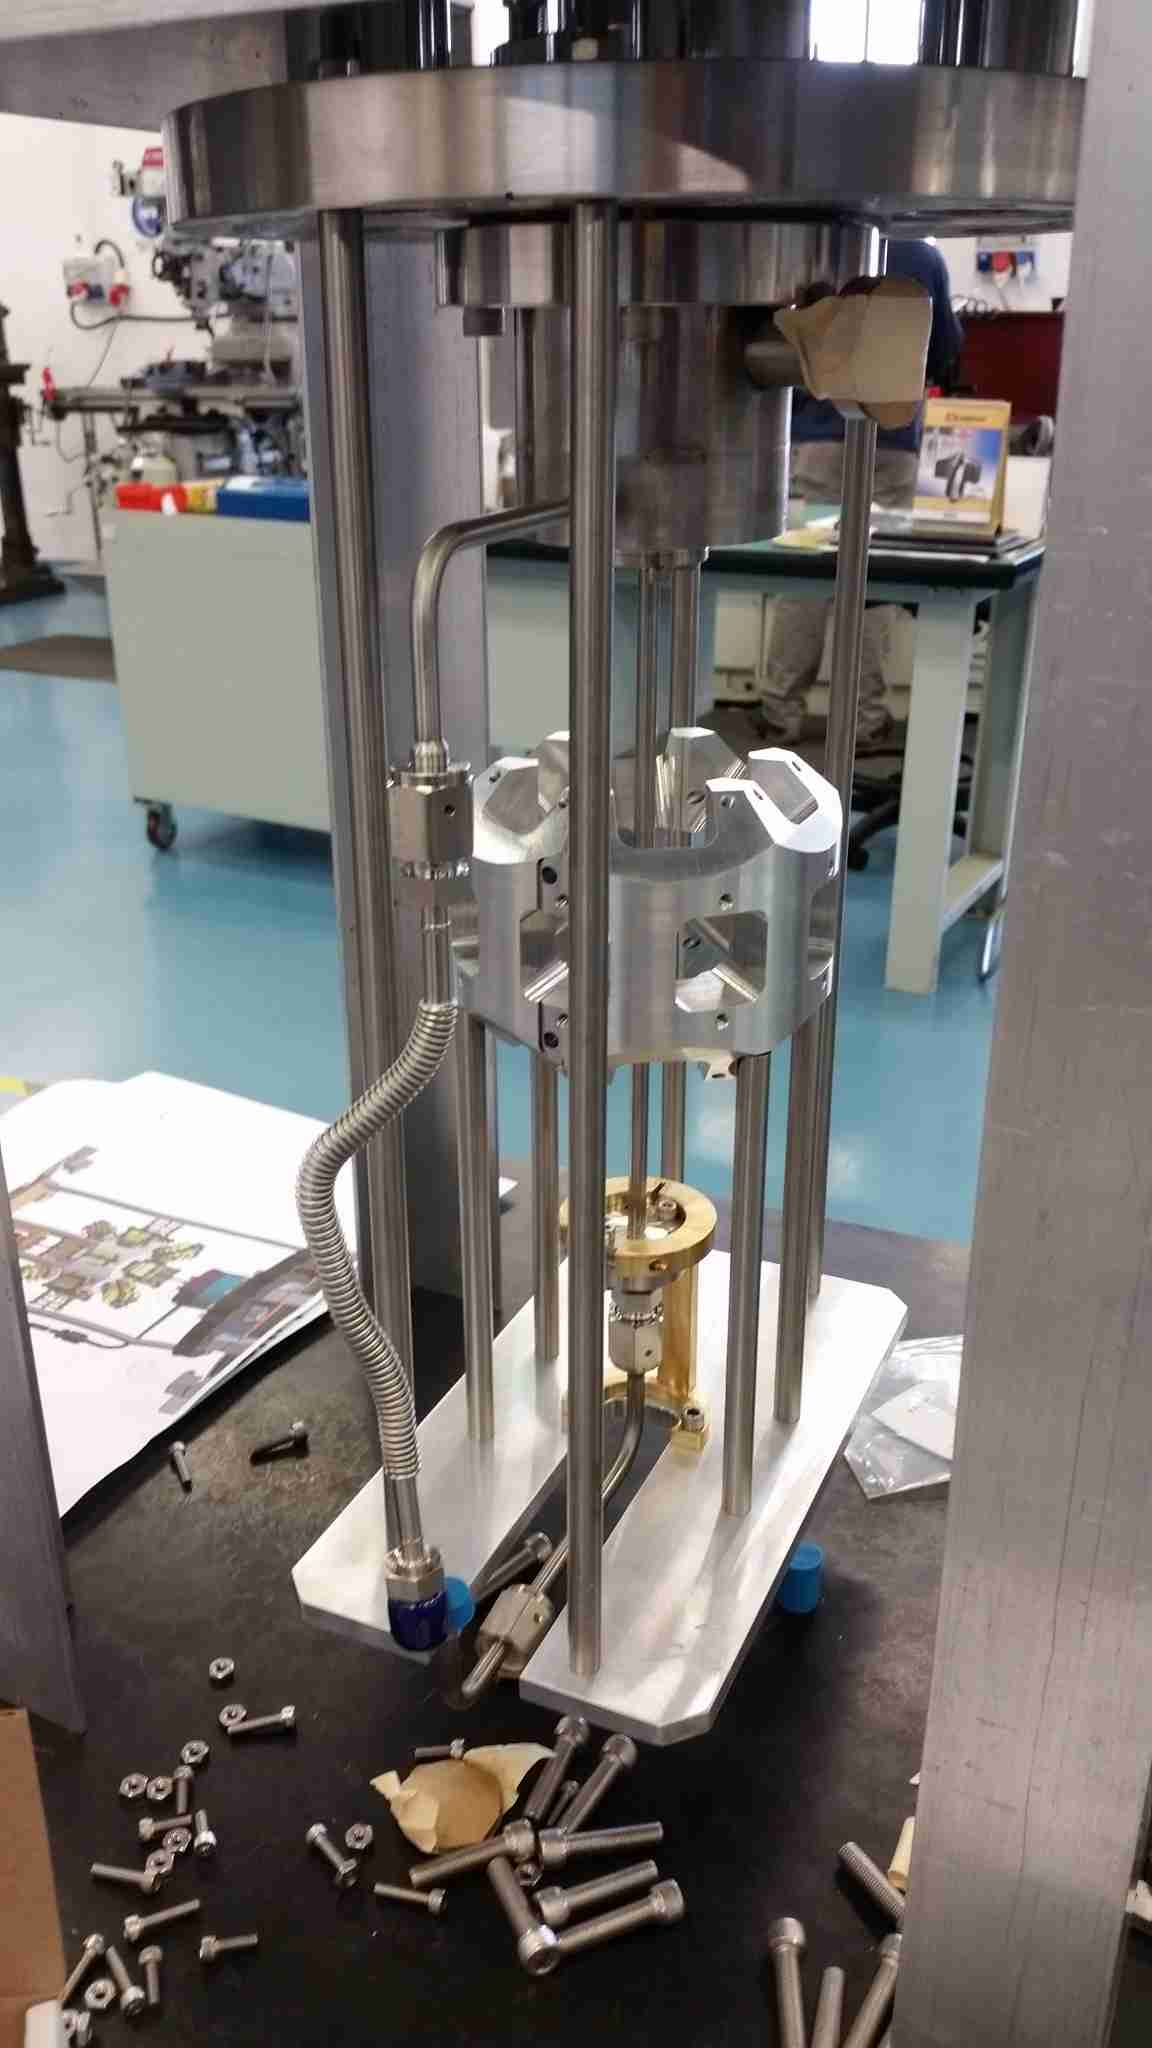
\includegraphics[width=\textwidth , height=0.35\textheight]{fig/detReal_small.jpg}}% Here is how to import 
\end{minipage}	
\mycaption[Detector part]{\label{fig:detector}(a) CAD design of the detector part. (b) First mounting of the 
detector part, still not connected to the rest of the system.}
\end{figure}


\subsection{The data acquisition system }
\label{sec:DAQ}

%%%%%%%%%%%%%%%%%%%%%%%%%%%%%%%%%%%%%%%%%%%%%%%%%%%%%%%%%%%%%%%%%%%%%%%%%%%%%%%%%%%%
%by MMdevi. Last modified July 2, 2017.
%%%%%%%%%%%%%%%%%%%%%%%%%%%%%%%%%%%%%%%%%%%%%%%%%%%%%%%%%%%%%%%%%%%%%%%%%%%%%%%%%%%%


The DAQ system is heterogeneous using both 
NIM and VME electronic modules. The data readout is being carried out through a PCIe card \footnote{CAEN A3818 PCIe}  connected via an optical link to a VME controller\footnote{CAEN V2718 VME controller}. A schematic layout of the DAQ system is shown in Fig.~{\ref{Fig:DAQscheme}}. 

The PMTs are ramped up to +800V (the maximum is +900V) using VME high voltage distributor module\footnote{iseg VDS18130p : 
24 independent channels positive polarity voltage distributer}. The raw pulses from the PMTs are amplified and shaped using 
two PMT preamplifiers\footnote{Phillips 776. 16 independent and direct-coupled amplifiers channels}. The preamplifier operates 
from DC to 275 MHz and produces two identical 50 $\Omega$ non inverting outputs with voltage gains of 10 for each PMT channel. One 
of the outputs is converted into a digital signal by an ADC\footnote{CAEN ADC V1742: switched capacitor digitizer}, and the other to 
binary signals using two discriminators\footnote{CAEN V895 16 channel leading edge discriminator}.

%%%%%%%%%%%%%%%%%%%%%%%%%%%%%%%%%%%%%%%%%%%%%%%%%%%%%%%%%%%%%%%%%%%%%%%%%%
\begin{figure}[h]
   \centering
   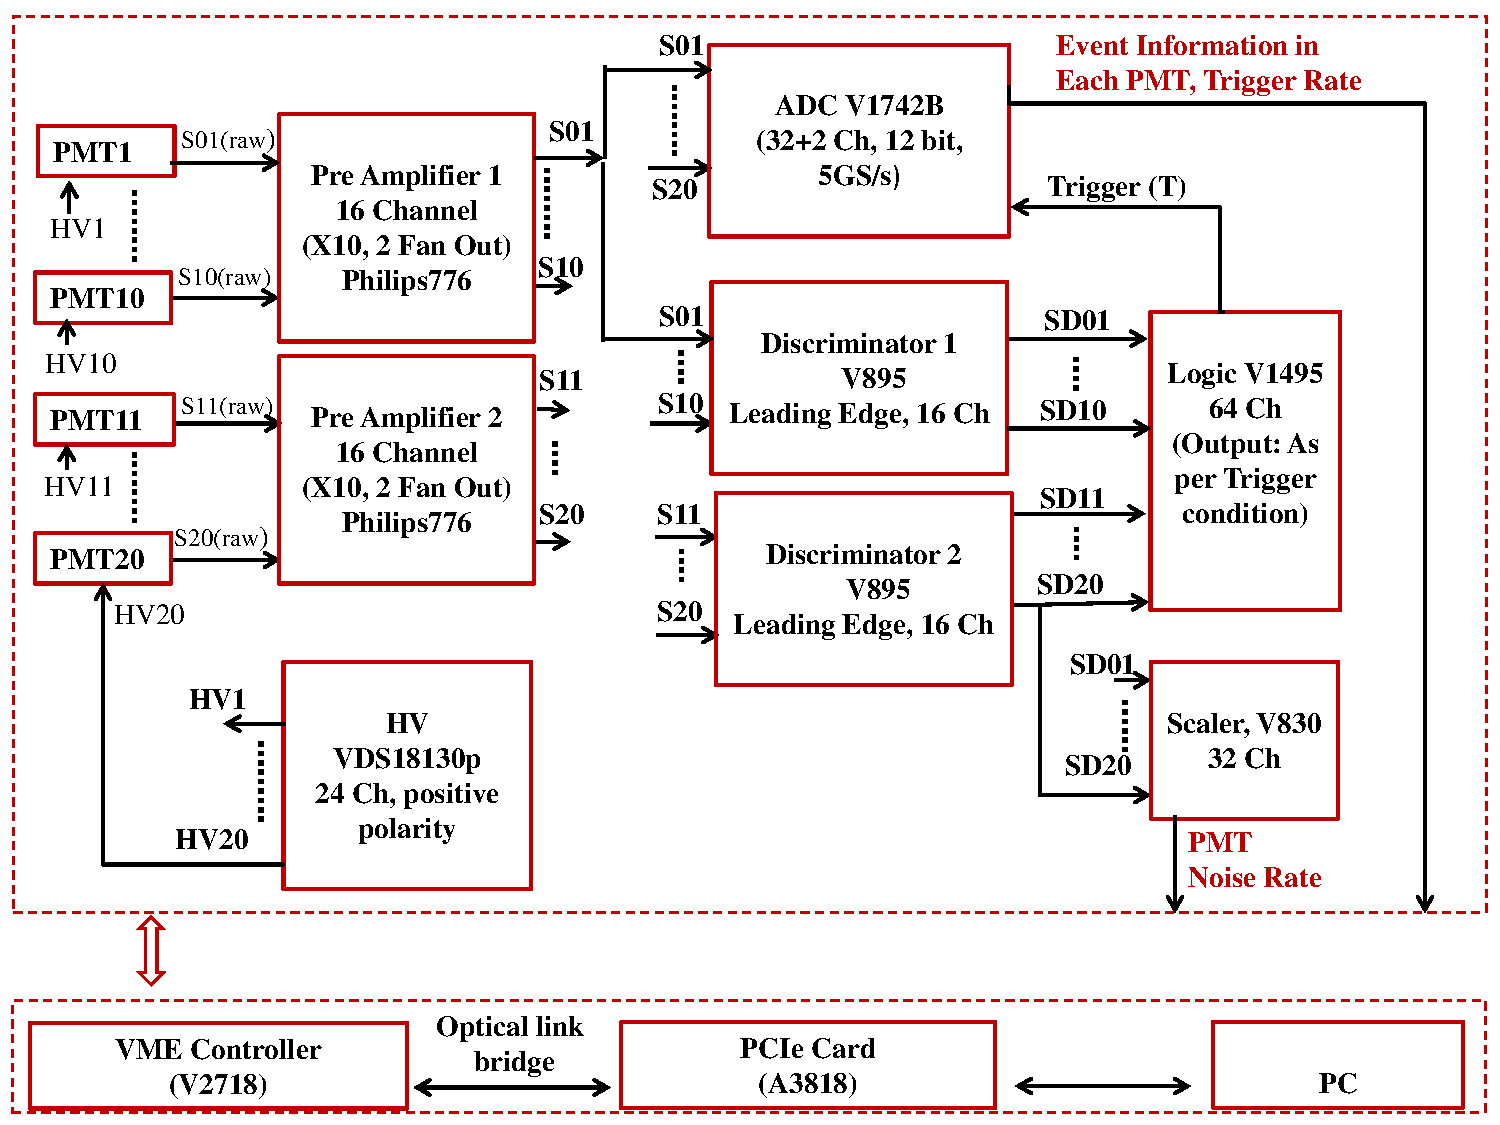
\includegraphics[width=0.85\textwidth]{fig/DAQscheme.pdf}
   \mycaption[DireXeno DAQ schematics]{The schematic of the data acquisition system of DireXeno. The 			signal coming from 20 PMTs ({\it i} = 1 -- 20) and the subsequent electronic channels to record the events once triggered. Where S{\it i}(raw) is the raw electrical pulse output of the PMTs, S{\it i} are the amplified pulses, and SD{\it i} are the binary outputs from the discriminator \RanComment{Why is VME controller in lower box }. 
}
   \label{Fig:DAQscheme}
\end{figure}
%%%%%%%%%%%%%%%%%%%%%%%%%%%%%%%%%%%%%%%%%%%%%%%%%%%%%%%%%%%%%%%%%%%%%%%%%%%


The ADC consists of two 12bit 5GS/s switched capacitor digitizer sections, 
each of them with 16+1 channels, based on DRS4 chip. The dynamic range of the input signal is 1 
Vpp with an adjustable DC offset. This module constantly samples (5GS/s, 2.5 GS/s or 2 GS/s) either bipolar or unipolar analog input 
signals, and records them into circular 
analog memory buffers. Once triggered, all analog memory 
buffers are frozen and digitized into a digital memory buffer 
with a 12 bit resolution. 

The binary output signals from the discriminator are duplicated and fed to 

the logic module\footnote{CAEN V1495: FPGA based general purpose VME board} and to a scaler\footnote{CAEN V830: 16 channel scalar}. 
A global majority trigger is generated in the logic module with the coincidence of any two out of the twenty PMTs within a time window of \RanComment{XXX\,ns}. The event information and trigger rate are read from the ADC, while the individual PMTs trigger rate from the scaler. Further analyses of the relevant events are carried out offline.



\section{Optical properties of the sphere }
\label{sec:opt}


The central component of the experiment is the HPFS sphere, which holds the LXe target, located in the center of the detector system. The sphere is made of two Corning HPFS 8655 hemispheres attached by a UV transparent glue. The refractive index of this HPFS is 1.58 at 185 nm, matching to the LXe one, which is 1.61. Hence, there is minimal diffraction from the original direction of the photons as they transit from the LXe target to the sphere. The refractive index at various wavelengths are shown in Fig.~\ref{fig:hpfsRIcalibration} (left panel).


The HPFS transparency to VUV photons is an extremely crucial parameter for setting the sphere's dimensions (inner and outer radii). 
Therefore, the transmittance of an HPFS sample was measured, using a VUV monochromator light source. The measured transmittances as a function of wavelength are shown in Fig.~\ref{fig:hpfsRIcalibration}~(right panel). The transmittance of the sample at 178~\,nm, is$\sim98.7$\,\%/cm.  

\begin{figure}
\centering
\begin{minipage}[c]{0.45\textwidth}
\subbottom[]{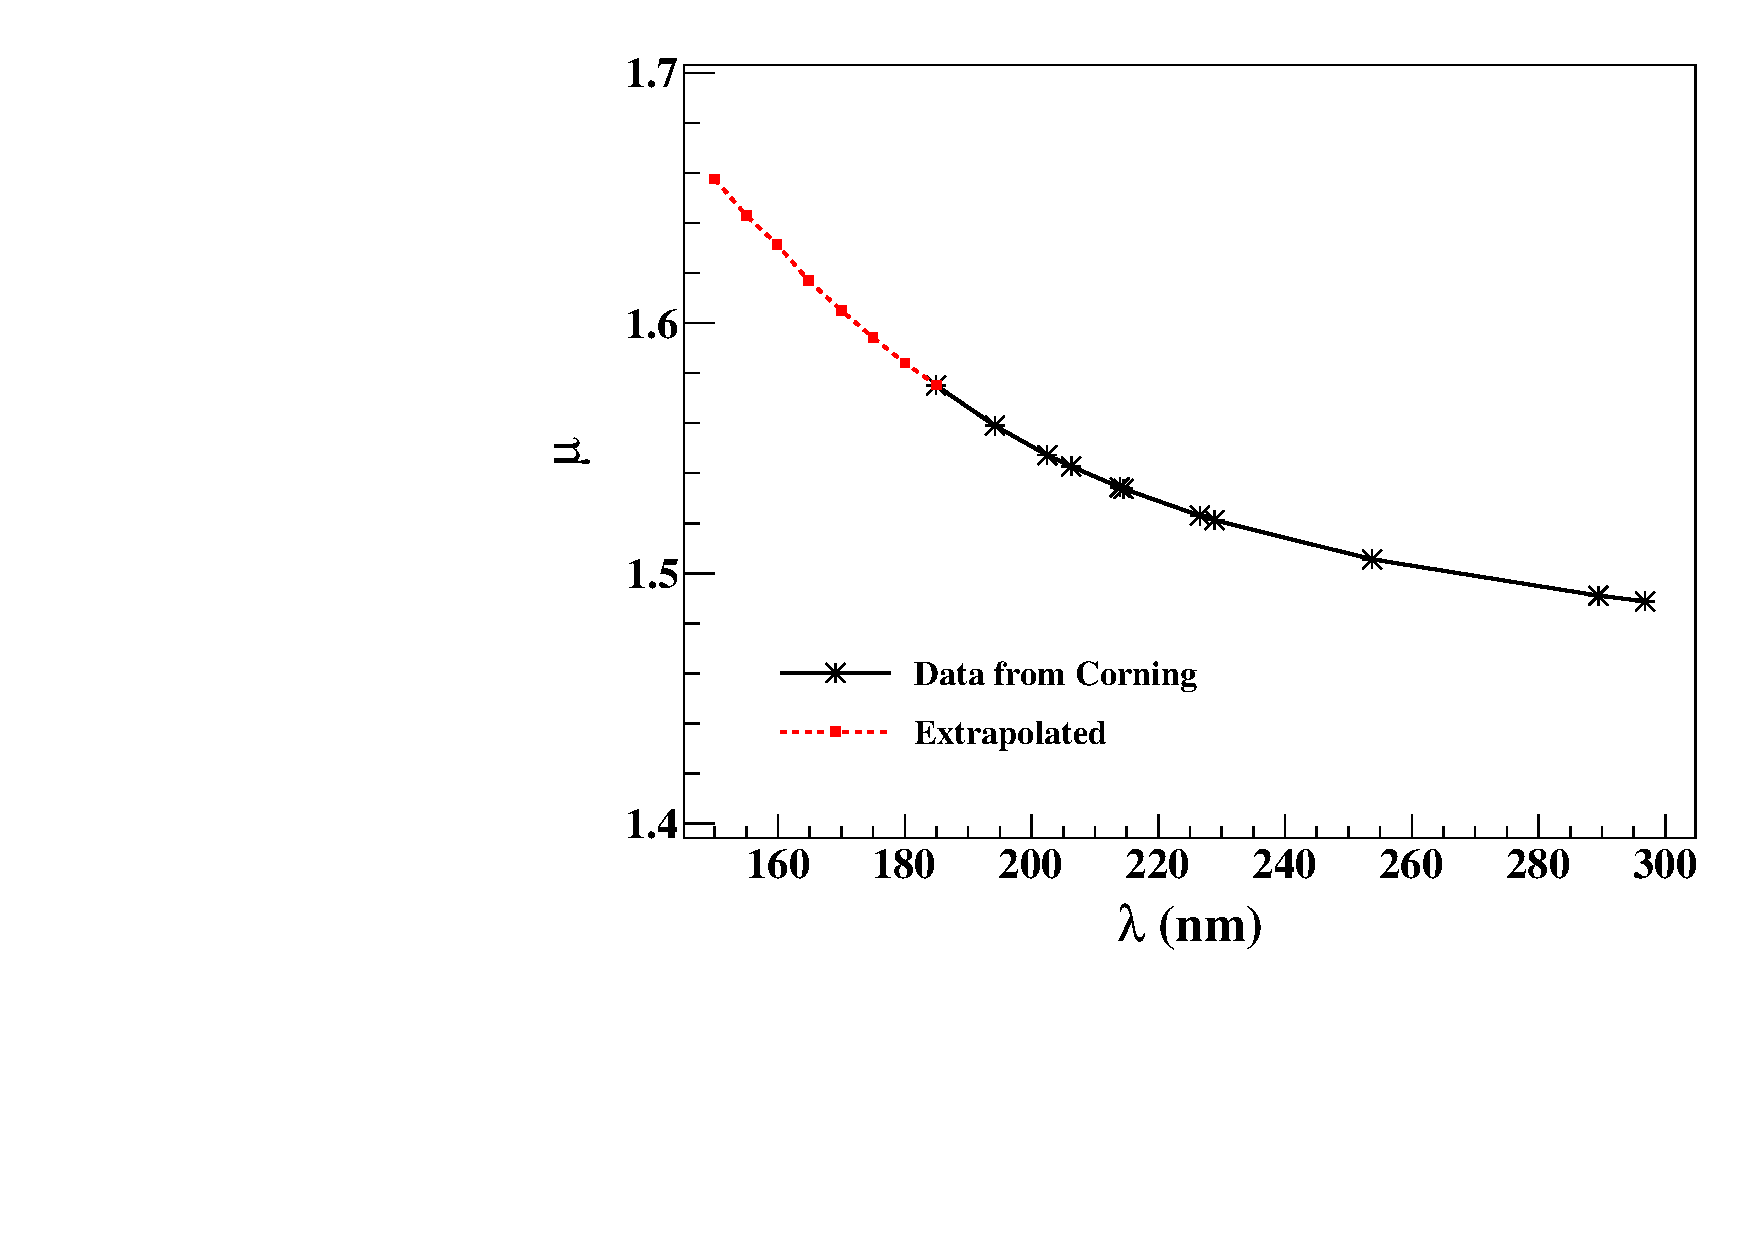
\includegraphics[width=\textwidth]{fig/RI-calibration.pdf}}% Here is how to import 
\end{minipage}	
\begin{minipage}[c]{0.45\textwidth}
\subbottom[]{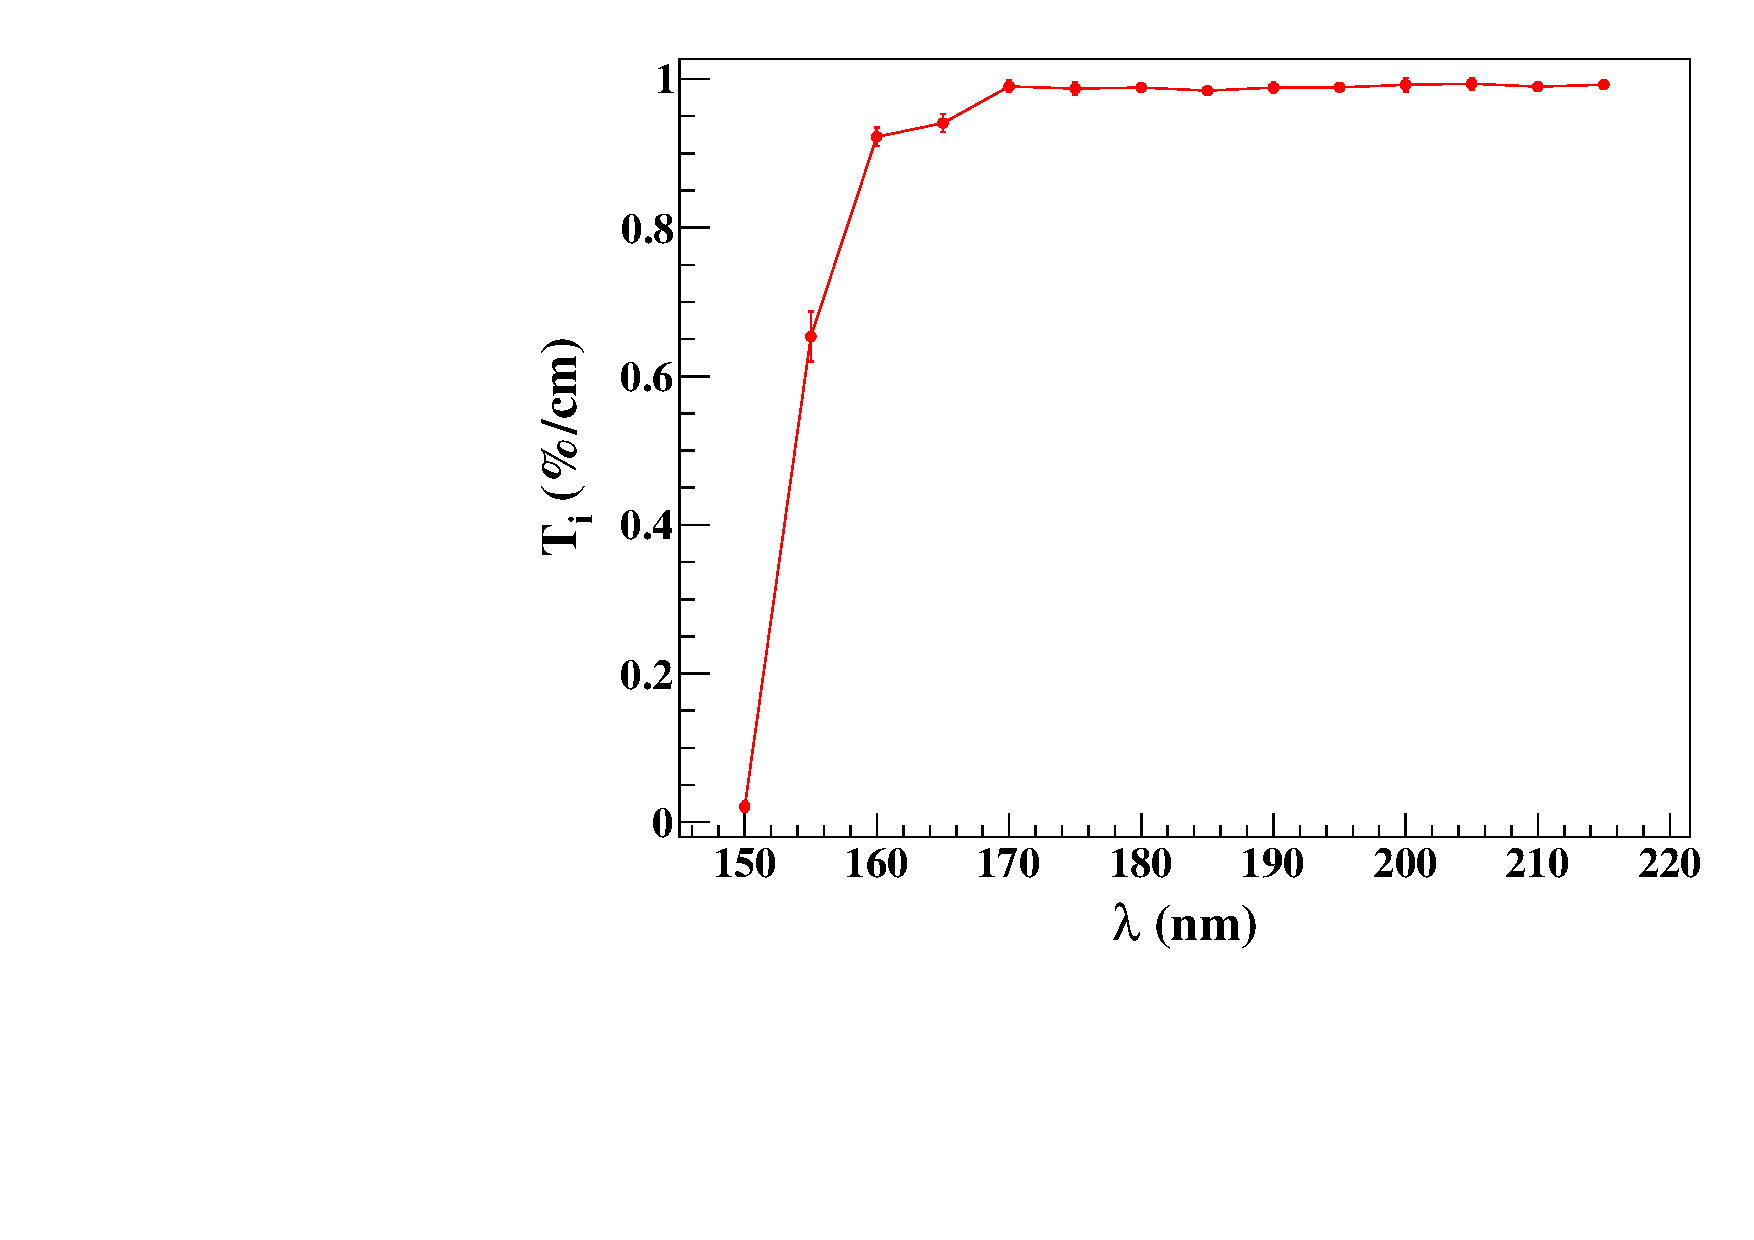
\includegraphics[width=\textwidth]{fig/IntTransmittance.pdf}}% Here is how to import 
\end{minipage}	
 \mycaption[Some relevant characteristics of HPFS-8655.]{Some relevant characteristics of HPFS-8655. (a) The refractive index as provided by corning and 
   extrapolated to relevant wavelength range. (b) The internal transmittance ($T_{i}$). \RanComment{Say something about the error bars}
   \label{fig:hpfsRIcalibration}}
\end{figure}

The sources that will be used for exciting the xenon, and creating the supperradiance (signal) as well as the standard emission (background), will be $^{137} \mathrm{Cs}$ 
(E$_\gamma$=662 keV) and $^{57} \mathrm{Co}$( E$_\gamma$= 122keV \& 136 keV) for ER with mean free path of $\sim4$\,cm and $\sim1$\,cm respectively. For NR $^{241}$AmBe , D-D neutron generator, or neutron produced in an accelerator will be used. 

Using a GEANT4 based simulation~\cite{AGOSTINELLI2003250} studying the path of the scintillation photons the sphere dimensions are optimized. The shell should be thick enough to reduce internal reflections, but not 
too thick to attenuate the scintillation light. The LXe target bubble within should not be too large in order to avoid double scatters. The outer radius  is 3 cm, and the inner (the hollow space that holds the LXe) is 1 cm. 

\FloatBarrier
\section{Detector sensitivity}
\label{sec:sim}
%%%%%%%%%%%%%%%%%%%%%%%%%%%%%%%%%%%%%%%%%%%%%%%%%%%%%%%%%%%%%%%%%%%%%%%%%%%%%%%%%%%%%%%%%%%%%%%%%%%%%%%%%%%%%%%%%%%%%%%%
The sensitivity of the detector is estimated by its ability to identify an anisotropic component in the scintillation photons emission pattern (signal), over the isotropic one (background). The photon emission pattern is modeled using a combination of isotropic emission and one or two beams:
\begin{equation}
\mathcal{F}(\theta,\phi) = (1-r_{aniso}) \cdot f_{iso} + r_{aniso}\cdot\left[r_1 f_G(\sigma_1) + r_2 f_G(\sigma_2) \right], 
\end{equation}  
where  $f_{iso}$ is the PDF of an isotropic emission, $f_G$ is a PDF of a Gaussian distribution with half width $\sigma$. $r_{aniso}$ is the anisotropic emission fraction, and $r_{1,2}$ are the relative beams intensities. The first beam direction is random, and the second's is either random 
(''uncorrelated``) or opposite to the first's (''correlated``). The different emission patterns used here are summarized in Table~\ref{tab:AnisoPattern}.
 
\begin{table}[h]
  \centering
  \caption{Anisotropic emission patterns. For all patterns $r_{aniso}$ = 0.1}
  \label{tab:AnisoPattern}
  \begin{tabular}{|c |c |c|cc|cc|c|}
  \hline
  Pattern no. & No. of beams & type & \multicolumn{2}{c|}{Beam half widths}& \multicolumn{2}{c|}{Signal fractions} & $N^{'}$ \\
 % \hline
  &              &      &  $\sigma_1$ & $\sigma_2$   &  $r_1$ & $r_2$ &   \\
  \hline
  1 & 1 & single beam & $5^{0}$ & - & 1 & 0 & 3200\\
  %\hline
   2 & 1 & single beam & $15^{0}$ & - & 1 & 0 & 4630\\
  %\hline
   3 & 2 & correlated & $5^{0}$ & $5^{0}$ & 0.5 & 0.5 &  4520  \\
  %\hline
   4 & 2 & correlated & $15^{0}$ & $15^{0}$ & 0.5 & 0.5 & 9770  \\
  %\hline
   5 & 2 & uncorrelated & $5^{0}$ & $5^{0}$ & 0.5 & 0.5 & 9370\\
  %\hline
   6 & 2 & uncorrelated & $5^{0}$ & $10^{0}$ & 0.5 & 0.5 & 19500\\
  %\hline
   7 & 2 & uncorrelated & $15^{0}$ & $15^{0}$ & 0.5 & 0.5 & 28200\\
  %\hline
   8 & 2 & uncorrelated & $10^{0}$ & $30^{0}$ & 0.5 & 0.5 & 49900\\
  %\hline
   9 & 2 & uncorrelated & $10^{0}$ & $30^{0}$ & 0.2 & 0.8 & 56000\\
  %\hline
    10 & 2 & uncorrelated & $30^{0}$ & $10^{0}$ & 0.2 & 0.8 & 43000\\
  \hline
 \end{tabular}
\end{table} 
 
 

A GEANT4 based simulation is used to model the detector system, generate photons, propagate them through the detector, and obtain a PMT hit pattern. The photons detected at the 
PMTs are mapped and put through a statistical test to check the detector's sensitivity towards the different emission patterns.

The relevant geometrical and optical parameters, which are used in the simulation, are listed in Table~\ref{tab:OptPar}. 
The scintillation light produced in a particular 
event is emitted by a cloud of excimers. This cloud is assumed to have a linear size much smaller than that 
of the optical system. Therefore each event is simulated as a number of photons that are emitted from a point 
in the LXe with some emission pattern (see Table~\ref{tab:AnisoPattern}). The number of generated photons for each event is taken to be Poisson(50), which correspond to an energy deposition of $\sim2.5\mathrm{keV}$  or $\sim7\mathrm{keV}$ for ER or NR respectively. The LXe target is much smaller than the mean free path of the source particles, and to 
account for that the events are uniformly generated in the LXe volume.
The probability for a photon being transmitted/reflected at a given surface is 
determined by Fresnel's equations, which include Snell's law for the transmitted light, 
and specular reflection for the reflected light. The boundary surfaces between different media
such as, the LXe--HPFS, HPFS--vacuum and vacuum--PMT, are assumed to be perfectly smooth, 
therefore enabling only specular reflection. 
The photons reaching the PMTs can either be detected, absorbed or reflected from the photocathode 
or PMT window. A simplified approach of the above possibilities is considered:
a photon reaching the PMT has a 30\% probability to be detected (since the PMTs have QE $\geq$ 30\%), 
50\% probability to get absorbed and 20\% probability to get specularly reflected. 

%%%%%%%%%%%%%%%%%%%%%%%%%%%%%%%%%%%%%%%%%%%%%%%%%%%%%%%%%%%%%%%%%%%%%%%%%%%%%%%%%%%%%%%
\begin{table}[h]
  \centering
  \caption{The parameters used in simulation}
  \label{tab:OptPar}
  \begin{tabular}{|l c||l c|}
  \hline
  Parameter & Value & Parameter & Value \\
  \hline
  LXe absorption length & 100 cm & HPFS shell inner radius & 1cm \\
  %\hline
  LXe scattering length & 35 cm & HPFS shell thickness & 2 cm\\
  %\hline
  LXe refractive index & 1.61  & PMT QE &  30\% \\
 % \hline
  LXe Scintillation wavelength & 178& PMT distance from center & 39 mm\\
 % \hline
  HPFS absorption length & 100 cm  & Number of PMT & 20 \\
  %\hline
  HPFS refractive index & 1.57 & PMT active area & 22mm $\times$ 22mm \\
  HPFS scattering length & $\infty$ & Invar tube diameter & 1 mm\\
  \hline
 \end{tabular}
\end{table}
%%%%%%%%%%%%%%%%%%%%%%%%%%%%%%%%%%%%%%%%%%%%%%%%%%%%%%%%%%%%%%%%%%%%%%%%%%%%%%%%%%%%%%%


The statistical fluctuation 
in the electronic signal generated in a PMT for a certain number of incident photon is 
taken into account. The R8520 PMTs have 20\% probability 
for double photoelectric emission for 178 nm photons, which is included in the simulation.
Each detected photon on a PMT is assigned a uniformly random position on the PMT surface. 
The direction of this point with respect 
to the center of the LXe sphere is defined as the incident direction of the photon. The direction information 
is then used to calculate the angles between all possible pairs of photon for any event and 
calculate the correlation between all angle pairs. \RanComment{Do you want to add fig of correlations iso and aniso?}

In order to quantify the anisotropicity of the emission, 
the angle correlation distribution of an anisotropic hit pattern is compared to that of the isotropic 
pattern. A $\chi^2$ test statistics is used where the reduced $\chi^2$ is defined as: 

\begin{equation}
\chi^2_\nu = \frac{1}{\nu} \sum^{\nu}_{i=1} \frac{(O_i - E_i)^2}{E_i},
\label{redchi2}
\end{equation}

where $E_i$ is the expected number of entries for an isotropic emission obtained from a sample of $10^5$ simulated events. 
$O_i$ is the observed number of entries, and $\nu$ is the total number of angle correlation bins 
which is also the degree of freedom. Sixty bins of identical width are used.


To asses the needed exposure to claim discovery assuming one of the   pattern mentioned above, $10^4$ data sets are generated and tested against the null hypothesis. This is repeated for increasing number of events between $1-4000$ assuming different values of the anisotropy fraction ($r_{aniso}$). The <$\chi^2_\nu$> 
and its 2$\sigma$ band for pattern 1, assuming $r_{aniso} =0.1$ overlaid with the corresponding values  for an isotropic emission are shown in Fig.~\ref{fig:pattern1}.  
The values of $N^{'}$, required to claim $5\sigma$ discovery, for different values of $r_{aniso}$ are calculated for each pattern as illustrated in Fig.~\ref{fig:convergence}.
The number of events 
$N^{'}$ for $r_{aniso} =0.1$ are summarized in Table~\ref{tab:AnisoPattern} for all emission patterns.

A simulation with two typical sources that emit isotropically, a 10 $\mu$Ci $^{137}Cs$ (662\,keV gamma), and a 2.7 $\mu$Ci AmBe ( 5\,MeV neutron), shows that for an average yield of 
50photons/event,  the rate of events in the detector is: $1.25\times10^{4}$\,events/day for NR and 625\,events/day for ER. 
Therefore a system that can operate stably for few weeks 
is expected to do reasonable measurements for ER and NR events.


%%%%%%%%%%%%%%%%%%%%%%%%%%%%%%%%%%%%%%%%%%%%%%%%%%%%%%%%%%%%%%%%%%%%%%%%%
\begin{figure}[h]
\centerline{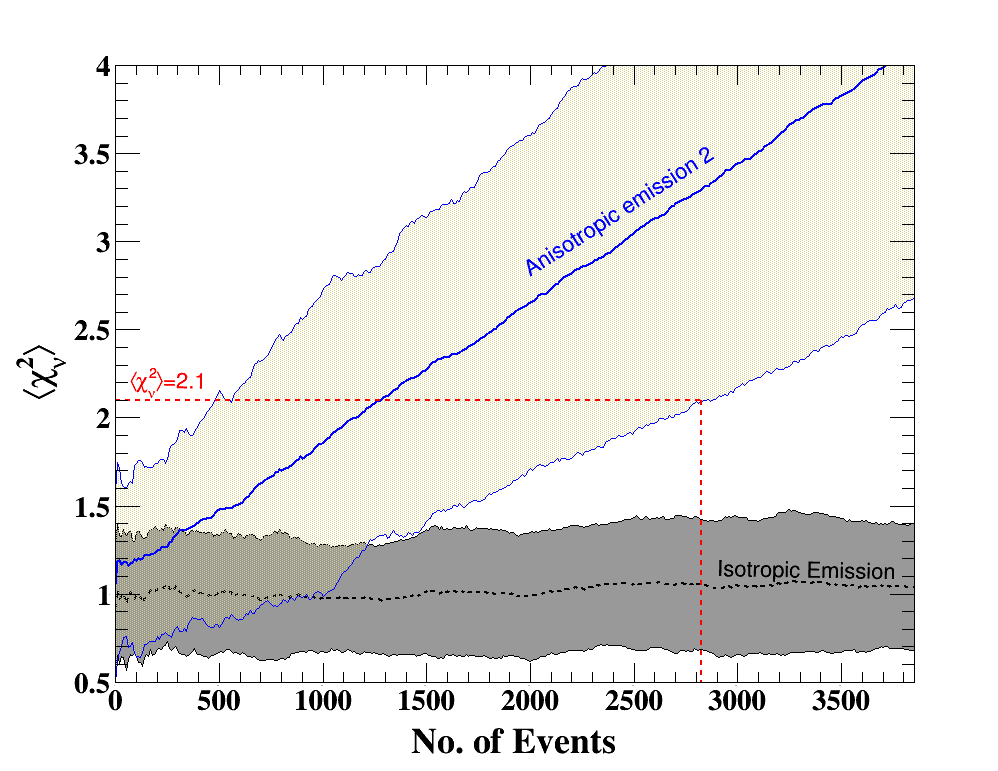
\includegraphics[width=0.5\linewidth]{fig/Pattern1.png}}
\mycaption[<$\chi^2_\nu$> test example.]{<$\chi^2_\nu$> and its $2\sigma$ band for isotropic emission (black) and for pattern 2 (blue). The <$\chi^2_\nu$> for 
isotropic emission fluctuate around 1 with $\sigma$ = 0.2 which is consistent with 
the expected value of $\frac{1}{\sqrt{30}} \equiv 0.18$ for reduced $\chi^2$ distribution 
with 60 degrees of freedom. $\sim3000$ events are needed to claim  5$\sigma$ discovery ($\chi^2_\nu=2.1$) for this emission pattern}
\label{fig:pattern1}
\end{figure}
%%%%%%%%%%%%%%%%%%%%%%%%%%%%%%%%%%%%%%%%%%%%%%%%%%%%%%%%%%%%%%%%%%%%%%%%%%%%

%%%%%%%%%%%%%%%%%%%%%%%%%%%%%%%%%%%%%%%%%%%%%%%%%%%%%%%%%%%%%%%%%%%%%%%%%
\begin{figure}[h]
\centering
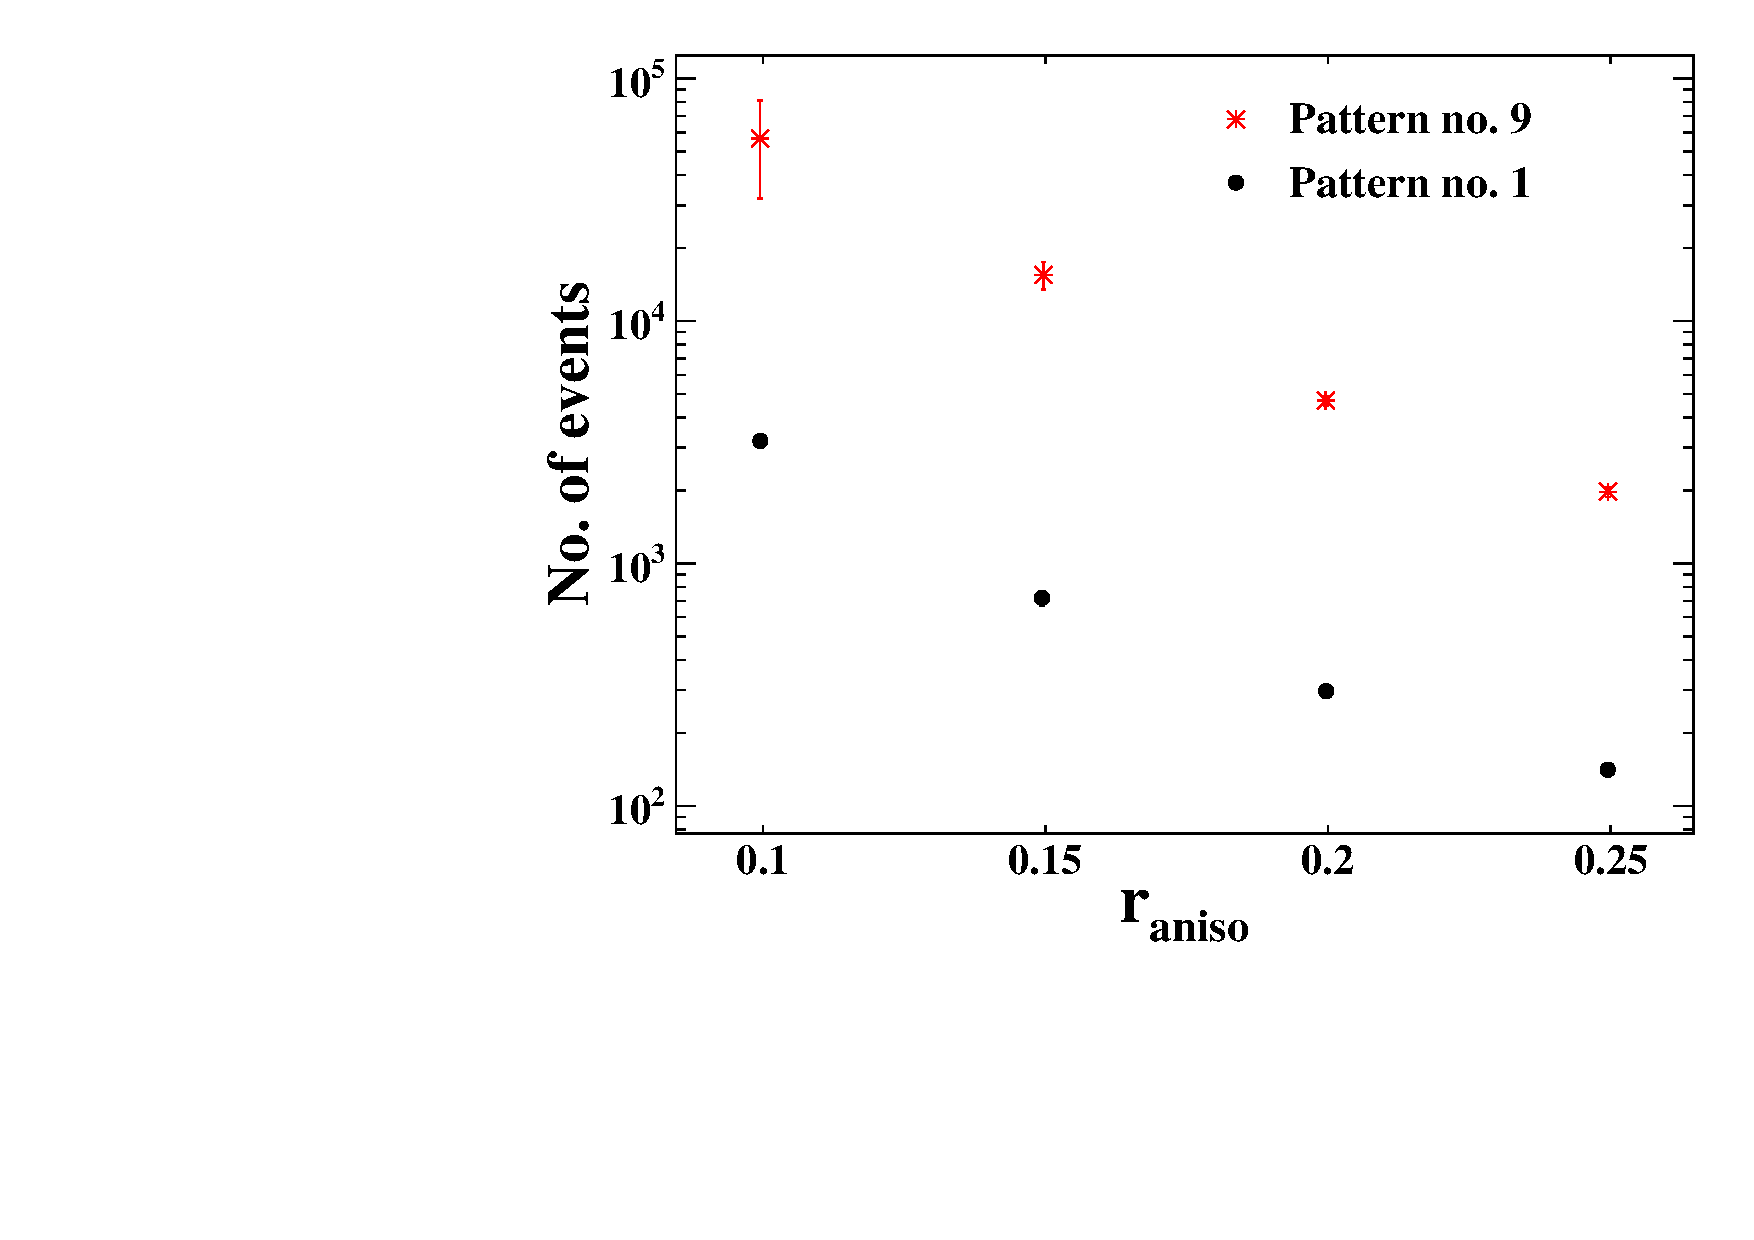
\includegraphics[width=0.45\linewidth]{fig/ConvergenceVsRaniso.pdf}
\mycaption[Simulation of Number of events for discovery ]{The number of events needed for each emission pattern to achieve $5\sigma$ presented only for pattern 1 and 9. Here 
$r_{aniso}$ = 0.1. for four different values of $r_{aniso}$.}
\label{fig:convergence}
\end{figure}
%%%%%%%%%%%%%%%%%%%%%%%%%%%%%%%%%%%%%%%%%%%%%%%%%%%%%%%%%%%%%%%%%%%%%%%%%%%%

\section{Summary}
\label{sec:Driexeno_summary}

The setup of Direxeno, an experiment to measure the spatial and temporal distribution of LXe scintillation, has 
been presented. The system consists of 4 main building blocks (gas handling, cryogenic, detector, 
and DAQ), each of which can be exchanged without altering others allowing significant flexibility 
and modularity. Each of the building blocks has been described in detail, with emphasis on the design 
and components.

The sensitivity of the setup to different postulated non isotropic emission patterns are studied using MC simulations. For the patterns studied, a run--time of 2-3 weeks is required using typical radioactive 
sources. Therefore the system is designed to maintain stability over a reasonable time period.

Using DireXeno, effects like superradiance or any other non-linear scintillation can be measured. 
Measuring the correlation between the direction of the emission and the direction of the radioactive 
source, may lead to directionality measurement which will allow enhanced statistical modeling of 
background and improved sensitivity in DM experiments.



